\section{File-Upload}

Als Bewerber können die Lösungen zu den einzelnen Aufgaben des Assessments in Form von Dateien abgegeben werden, wobei
es sich meistens um Programmcode oder Bilder handelt. Dazu wird ein File-Upload benötigt, der in neueren Ruby on Rails Versionen über die mitgelieferte \emph{ActiveStorage} Bibliothek relativ einfach Integriert werden kann. 
ActiveStorage ist perfekt für die Cloud vorbereitet und die Integration von Amazon S3 ist bereits vorhanden. Die Konfiguration von ActiveStorage erfolgt über eine YAML-Datei.

\begin{figure}[H]
\begin{codebox}
\begin{minted}{yaml}
test:
  service: Disk
  root: <%= Rails.root.join("tmp/storage") %>

local:
  service: Disk
  root: <%= Rails.root.join("storage") %>

amazon:
  service: S3
  access_key_id: <%= ENV['AWS_S3_ACCESS_KEY_ID'] %>
  secret_access_key: <%= ENV['AWS_S3_SECRET_ACCESS_KEY'] %>
  bucket: <%= ENV['AWS_S3_BUCKET'] %>
  region: "eu-central-1"
\end{minted}
\end{codebox}
\caption{\label{fig:active-storage-config}Konfiguration von ActiveStorage über das \emph{config/storage.yml}}
\end{figure}

Für jedes Enviroment (development/test/production) kann dann Konfiguriert werden, was für ein Storage-Service verwendet werden soll.
Dazu wird z.B für Tests das lokale Verzeichnis \emph{tmp/storage} verwendet, welches nicht in das \gls{vcs} eingecheckt wird. So kann das
Upload-Feature überall genutzt werden und es wird keine dedizierte S3 Testinstanz benötigt.

Wie bereits im Diagramm \ref{fig:erd} ersichtlich, verwendet ActiveStorage gewisse Tabellen in der Datenbank, um die Uploads zu verwalten.
Sowohl der Schlüssel, der auf die eigentliche Datei im S3 verweist als auch sämtliche Metadaten wie Name, Dateigrösse oder Inhaltstyp werden in einem \emph{active\_storage\_blobs} gespeichert.
Die \emph{active\_storage\_attachments} Tabelle agiert als eine polymorphe Join-Tabelle, welche Referenzen auf ein Blob und das eigentliche Objekt (z.B auf die \emph{solution}) enthält. 
So sind mehrere Arten von Attachment-Beziehungen für ein einziges Model möglich.

Nun soll es möglich sein, mehrere Dateien zu einer \emph{solution} hochzuladen. Durch das alleinige Hinzufügen der \emph{has\_many\_attached} Funktion in das Model,
können nun Dateien über ein dediziertes Formularfeld hochgeladen werden. Damit dies auch mit mehreren Dateien auf einmal möglich ist,
wird das \emph{multiple} HTML-Attribut auf dem Input-Feld verwendet. 

\begin{codebox}
\begin{minted}{ruby}
class Solution < ApplicationRecord
  has_many_attached :uploads
  
  ...
end
\end{minted}
\end{codebox}

\begin{codebox}
\begin{minted}{ruby}
= simple_form_for([@task, @solution]) do |f|
    = f.input :uploads, input_html: { multiple: true }
    = f.button :submit
\end{minted}
\end{codebox}

Das Formular wird dann, wie man in der Formulardefinition erkennen kann, unter einen Task \enquote{genested} und auf dessen Detail-Seite gerendert.
So würde dieses Formular beispielsweise auf \emph{/tasks/275/solutions} posten und so eine neue Lösung für die entsprechende Aufgabe erstellen.

\begin{figure}[H]
  \centering
  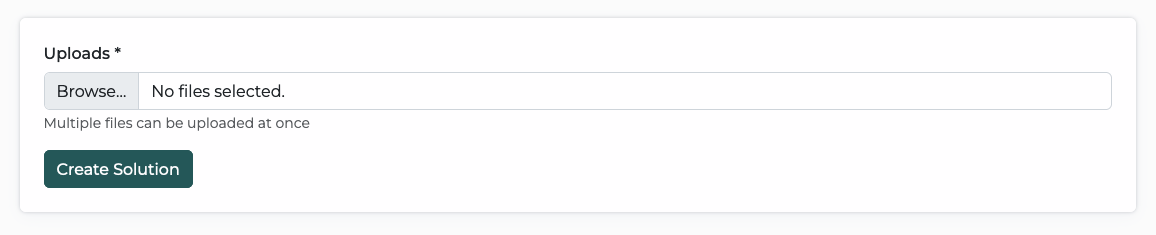
\includegraphics[width=\textwidth]{images/upload.png}
  \caption{\label{fig:solution-create}Formular für das Hochladen einer Lösung}
\end{figure}
